\documentclass[12pt,titlepage]{report}
\usepackage[authoryear,semicolon]{natbib}
\usepackage{mathptmx} 
\usepackage{pdfpages}
%\usepackage{chicago}
\usepackage[onehalfspacing]{setspace}
%\doublespacing
%\linespread{1.6}
\setstretch{1.5}
%\usepackage{figure}
\onehalfspacing
\usepackage[left=40mm,right=25mm,top=30mm,bottom=20mm,headsep=10mm]{geometry}
\geometry{a4paper}
\usepackage[titletoc]{appendix}
\usepackage{fnpara}
\usepackage{graphicx}
\usepackage{epstopdf}
%\usepackage{mathtools}
\usepackage{amsmath,amsfonts,amsthm,amssymb}
\usepackage{fancybox}

%\usepackage[active]{srcltx}
\usepackage{afterpage}
\usepackage[mathscr]{eucal}
\DeclareGraphicsRule{.tif}{png}{.png}{`convert #1 `dirname
#1`/`basename #1 .tif`.png}
%\usepackage{fancyhdr}
%\pagestyle{fancy}
%\fancyhf{}
%\rhead{ \leftmark}
%\rhead[\thepage]{\chaptermark}
%\lhead{Oyebamiji, O.K.}
%\cfoot{ \thepage}


\usepackage{setspace}
\usepackage[small]{caption}
\usepackage{color}
\usepackage{apalike}
%\usepackage{subcaption}
\usepackage{placeins}
\usepackage{epstopdf}
\usepackage{booktabs}
\usepackage{tikz}
\usepackage{subcaption}
%\usepackage{color,framed} %Utilisation des couleurs et de l'environnement shaded
%\definecolor{shadecolor2}{rgb}{.92,.92,.92} % choix de la teinte de ``shaded''
%\definecolor{shadecolor}{rgb}{.6,.95,.6} % choix de la teinte de ``shaded''
\usepackage[pagebackref=true,colorlinks=true, linkcolor=blue,anchorcolor=blue,citecolor=blue,filecolor=blue,menucolor=blue,
urlcolor=black,plainpages=false,pdfpagemode=UseThumbs,pdftitle={Titre},pdfauthor={oluwole},
pdfsubject={Thesis},pdfstartview=FitH]{hyperref} % Extensions PDF
%\def\pdfBorderAttrs{/Border [0 0 0] } % Options PDF (No border around Links)
%\usepackage[plainpages=false,backref=page,hypertexnames=true,linktocpage=true,colorlinks=true,citecolor=blue,linkcolor=blue]{hyperref}


%=========Standard sets===========:
\newcommand{\stsets}[1]{\mathbb{#1}}
\newcommand{\R}{\stsets{R}}
\newcommand{\N}{\stsets{N}}
\newcommand{\C}{\stsets{C}}

%===============Theorems etc.========================
%Paul
\newcommand{\bt}{{\bf t}}
\newcommand{\bB}{{\bf B}}
\newcommand{\bSigma}{{\bf \Sigma}}
\newcommand{\tbSigma}{{\tilde {\bf \Sigma}}}
\newcommand{\tbu}{{\tilde {\bf u}}}
\newcommand{\tbU}{{\tilde {\bf U}}}
\newcommand{\bh}{{\bf h}}
\newcommand{\bH}{{\bf H}}
\newcommand{\bD}{{\bf D}}
\newcommand{\bU}{{\bf U}}
\newcommand{\bu}{{\bf u}}
\newcommand{\bZ}{{\bf Z}}
\newcommand{\bz}{{\bf z}}
\newcommand{\bC}{{\bf C}}
\newcommand{\bc}{{\bf c}}
%%
\newcommand{\bx}{{\bf x}}
\newcommand{\bX}{{\bf X}}
\newcommand{\by}{{\bf y}}
\newcommand{\bY}{{\bf Y}}
\newcommand{\bE}{{\bf E}}
\newcommand{\bW}{{\bf W}}
\newcommand{\tbx}{{\tilde {\bf x}}}
\newcommand{\tbX}{{\tilde {\bf X}}}
\newcommand{\tby}{{\tilde {\bf y}}}
\newcommand{\tbY}{{\tilde {\bf Y}}}
\newcommand{\hbX}{{\hat {\bf X}}}
\newcommand{\hbY}{{\hat {\bf Y}}}
\newcommand{\hby}{{\hat {\bf y}}}
\newcommand{\ty}{{\tilde {y}}}
\newcommand{\hy}{{\hat {y}}}
\newcommand{\bs}{{\bf s}}


\newcommand{\bLambda}{\mathbf{\Lambda}}
\newcommand{\bGamma}{\mathbf{\Gamma}}
\newcommand{\hbGamma}{\hat {\mathbf{\Gamma}}}

\newcommand{\bgamma}{{\boldsymbol{\gamma}}}
\newcommand{\bepsilon}{{\boldsymbol{\varepsilon}}}
\newcommand{\tbepsilon}{{\tilde{\boldsymbol{\varepsilon}}}}
\newcommand{\hbepsilon}{{\hat{\boldsymbol{\varepsilon}}}}
\newcommand{\bbeta}{{\boldsymbol{\beta}}}
\newcommand{\hbbeta}{{\hat{\boldsymbol{\beta}}}}
\newcommand{\btau}{{{\boldsymbol{\tau}}}}
\newcommand{\balpha}{{\boldsymbol{\alpha}}}
\newcommand{\bhalpha}{{\hat{\boldsymbol{\alpha}}}}


\theoremstyle{definition}
\newtheorem{definition}{Definition}
\theoremstyle{remark}
\newtheorem{remark}[definition]{Remark}
\newtheorem{example}[definition]{Example}

%\newtheoremstyle{mytheorem}{0.5cm}{0.2cm}{\slshape}{ }{\bfseries}{.}{}{}
%\theoremstyle{my theorem}
\newtheorem{Th}[definition]{Theorem}
%\newtheorem{Prop}[definition]{Proposition}
\newtheorem{lemma}[definition]{Lemma}
\newtheorem{Cor}[definition]{Corollary}
%\restylefloat{figure}

%==========Probabilistic===========:
%\renewcommand{\cite}{\shortciteN}
\renewcommand{\P}{\mathbf{P}}
\renewcommand{\Re}{\mathrm{Re\,}}
\renewcommand{\Im}{\mathrm{Im\,}}
%\newcommand{\Prob}[1]{\mathbf{P}\{#1\}}
\DeclareMathOperator{\E}{{\bf E}}
\DeclareMathOperator{\var}{{\bfvar}}
\DeclareMathOperator{\supp}{supp}
\DeclareMathOperator{\dist}{dist}
\DeclareMathOperator{\one}{{1\hspace*{-0.55ex}I}}
%\DeclareMathOperator{\one}{{\mathbf{1}}}
\newcommand{\Ind}[1]{\one_{#1}}
\newcommand{\cond}{\hspace*{1ex} \rule[-1ex]{0.15ex}{3ex}\hspace*{1ex}}

%==========Divers===========:
\DeclareMathOperator*{\ssum}{{\textstyle \sum}}
%small\sum for\sum\delta_x
\newcommand{\comp}{\mathbf{c}}
\newcommand{\mydot}{{\raisebox{.3ex}{$\scriptscriptstyle{\,\bullet\,}$}}}
%\newcommand{\myline}{\newline\underline{\hskip\textwidth}}
\newcommand{\mytimes}{\!\times\!}
\newcommand{\mytilde}{{\!\raisebox{-0.9ex}{$\tilde{\ }$}}}
\renewcommand{\epsilon}{\varepsilon}
\renewcommand{\vec}[1]{\mathbf{#1}}
%\renewcommand{\phi}{\varphi}
\newcommand{\ti}{\to\infty}
\newcommand{\ssp}{\hspace{2pt}}
\newcommand{\seg}{see, \hbox{e.\ssp g.,}\ }
\newcommand{\ie}{\hbox{i.\ssp e.}\ }
\newcommand{\eg}{\hbox{e.\ssp g.,}\ }
\newcommand{\cf}{\hbox{c.\ssp f.}\ }
\newcommand{\etc}{\hbox{etc.}\ }
\newcommand{\iid}{\hbox{i.\ssp i.\ssp d.}\ }
\newcommand{\as}{\hbox{a.\ssp s.s}\ }
\newcommand{\viz}{\hbox{viz.}\ }
\renewcommand{\bibname}{References}
\renewcommand{\abstractname}{Abstract}


%\pagenumbering{roman}

\begin{document}
\chapter{Emulator as a tool for upscaling LAMMPS model outputs}

\section{Introduction}
We shall briefly describe requirements and strategies for building a simple emulator of LAMMPS model outputs including how to apply the emulator to address the upscaling problem. 

%The main issue we address here is the upscaling problem that involves transferring of information from one spatial or temporal scale to another one.
There is a common assumption that to identify crucial features and model water treatment plant on a large scale, and there is a need to understand the interactions of microbes at fine resolution based models that could provide the best available representation of micro scale responses. The challenge then becomes how we can transfer this small-scale information to the macroscale process via a mesoscale in a computationally efficient and sufficiently accurate way, and to also probably quantified the associated risk or error in the process.

The macro scale characteristics of wastewater treatment plants are the consequences of microscale features of a vast number of individual particles that produce the floc \citep{l11}. In other words, the properties of cells or particles at a micro level is used for characterising the behaviour of wastewater treatment plant at a macro scale, even though there is a wide separation in their spatial and temporal dimensions at which their biological and physical processes take place. Flocs are the aggregation of microbes mixed with an adhesive material called EPS. The floc plays a strategic role in understanding the process involves in wastewater treatment plant. 

The complex nature of the transition from cellular level (microscale) to floc/biofilm (mesoscale) and to waste water treatment plant (macro-scale) introduce a scaling problem and a robust and coherent strategy is required to efficiently handle this multi-scale problem.
One useful approach to this challenge is the use of statistical emulators called metamodels. Emulation is a statistical technique for simplifying models that leads to reduced-form representations of complex models that are computationally much faster to run.

\section{Objectives}
The aim of this report is to describe how to use an emulator as an effective tool for understanding and incorporating microscale processes in a computationally efficient way into macroscale models. The emulator produced will be incorporated into the LAMMPS routine at mesoscale to produce a more refined LAMMPS model that are much computationally efficient for providing information on a large scale. The main issue we address here is the upscaling problem that involves transferring of information from one spatial or temporal scale to another one.

The fundamental question here is the development of statistical algorithms for emulation and calibration of complex multi-scale stochastic biological models (LAMMPS).
Emulation is an attempt to imitate the internal design of a simulator statistically. We shall describe the step for the construction of useful stochastic emulators. We will also address possible challenges of constructing good emulators in this project. 

The purpose of building an emulator is to facilitate other calculations that would be too computationally demanding using the simulator itself. In this project, emulator will be using mainly for 
\begin{itemize}
\item[(1)] Prediction /extrapolation to address the scale-up problem that arose due to LAMMPS models being too computationally expensive, so running LAMMPS models iteratively poses a problem and involve a computer run of several days which makes computational speed highly problematic for our study.

\item[(2)] Calibration of LAMMPS model parameters that shall involve using observational data to learn about uncertain parameters and initial conditions. 
\end{itemize}

We will highlight the strategy to address the first problem in this report. LAMMPS model is a stochastic simulator because running the simulator for the same input configuration gives different outputs and it is also dynamic in nature being a system that evolves over time and operates iteratively over fixed time steps. LAMMPS is a single-step simulator. A single run of LAMMPS model consists of a simulation over many time steps which requires much computer workload and time taken.

There are two different approaches to this problem. Firstly, we could emulate the simulator outputs (e.g., particles at the micro level) and use the emulator to link to the simulator at a mesoscale level for a floc/biofilm. This approach is currently not practicable owing to a large number of simulation data involves, although it could be possible to perform some forms of data reduction and pattern decomposition will even complicate the upscaling problem. The second approach that we adopt is to focus on the cluster of particles as a floc/biofilm and emulate their interested properties directly. 

The first critical task is to produce emulator for scaling up the micro level simulation to mesoscale levels. The LAMMPS models are run over many scenarios of initial conditions and input parameters that produce a large amount of high-dimensional simulation runs which is infeasible over the temporal support of interest with the current setting. Therefore, there is a need to introduce statistical emulator as a surrogate to efficiently transform the simulation at micro levels to useful information for floc modelling at the mesoscale. 

\section{The challenges}
The major challenges of NUFEB project, particularly for LAMMPS emulation is to be able to establish a good linear relationship between the particles and floc (particle-to-floc transition). For instance, emulation of floc or biofilm properties and shape from component particles at small-scale requires a bit of a careful strategy. The LAMMPS model is a bit more complicated to emulate easily because

\begin{itemize}
%The system is sufficiently complex
\item[(1)] The LAMPPS model is expensive to evaluate - we can not run them at every parameter combination of interest, which limit the amount of information we have.
\item[(2)] The LAMMPS model is stochastic and dynamic. 
\item[(3)] The model produce high-dimensional and multiple outputs.
\item[(4)] The model outputs are affected by few inputs.
\end{itemize}
Despite all these caveats, the good news is that there is a large number of literature that have addressed some of these problems, and we are applying suitable ones to our case. For instance, we are currently implementing parallel running of LAMMPS on a departmental HPC/ distributing computer especially for floc simulation that is taking a considerable amount of time.

%\cite{l2} Presents a broad range of techniques for measuring floc structural characteristics of size, shape and fractal dimension and also emphasise the role of floc size distribution and fractal dimension as the relevant parameters for activated sludge. \cite{l3} describes several techniques for characterizing the floc dimensions, including most common size measurements that are used in the literature for flocs  

%terms of a simpler, single-step simulator being run iteratively many times.
%What are the requirements for building the stochastic emulator under the NUFEB project? We shall describe mainly the procedure.
\begin{figure}[!ht] 
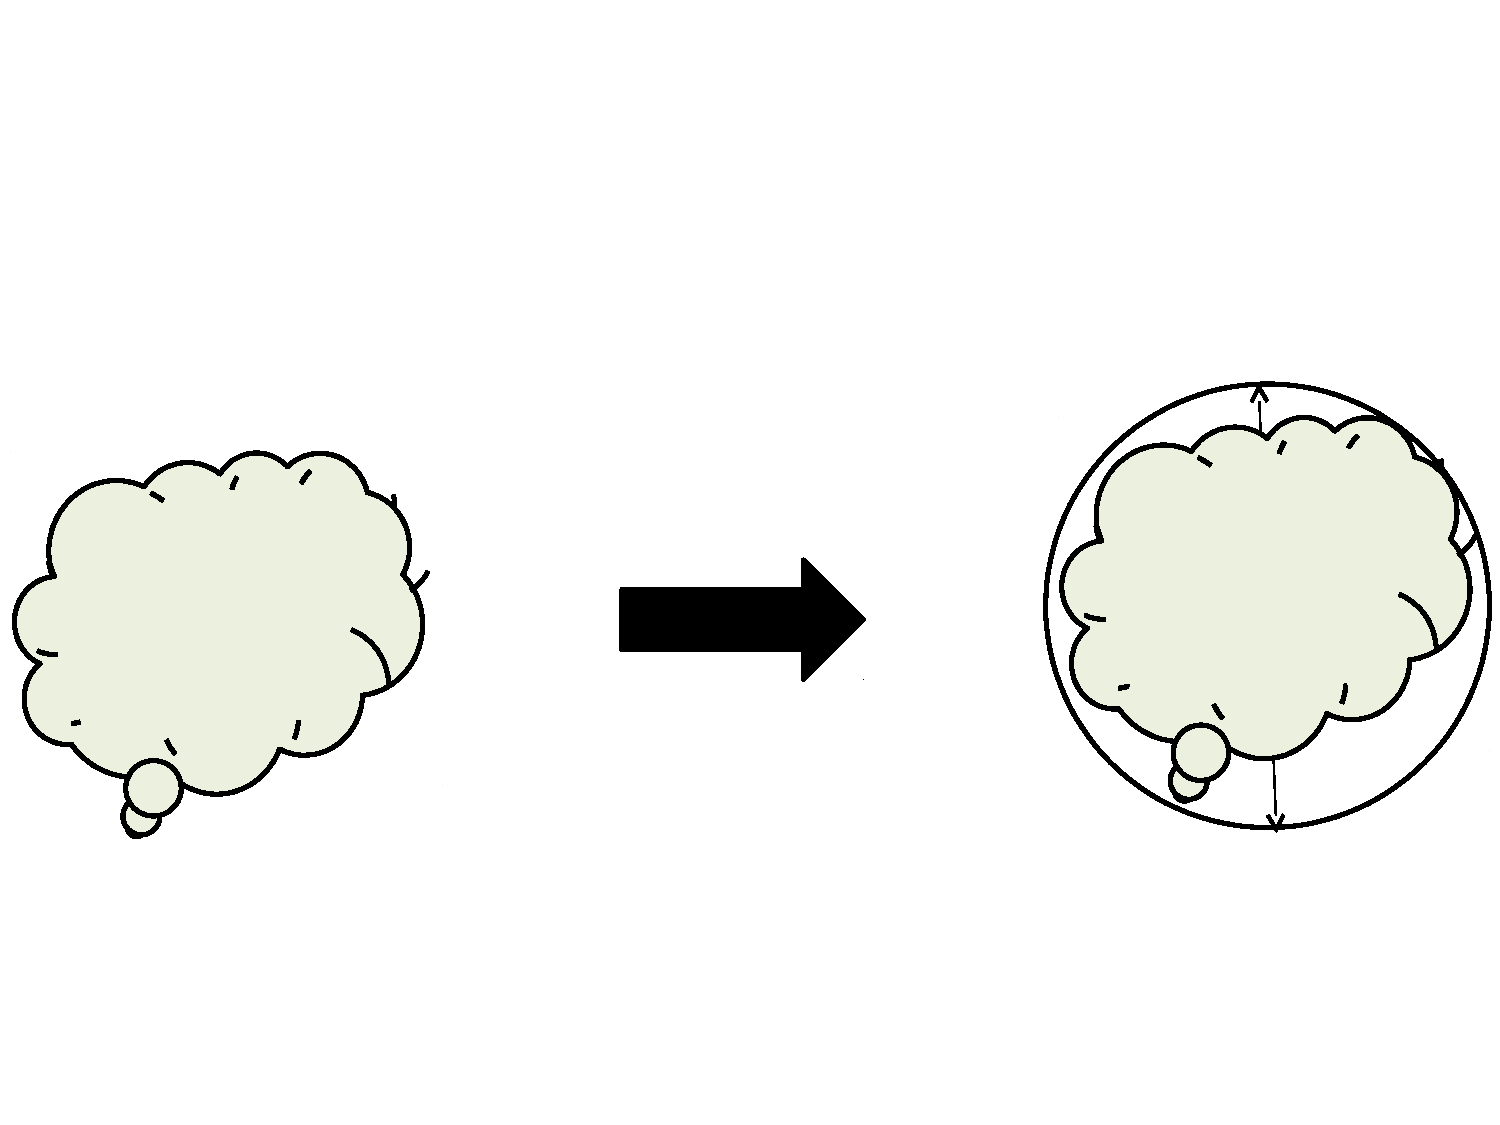
\includegraphics[width=1.1\textwidth]{diagram2}
\caption[]{Transformation of microscale particles to floc or biofilm at the mesoscale. Floc equivalent diameter is the diameter of the smallest sphere that circumscribes the outline of the projected floc.}\label{diag2}
\end{figure}

\begin{figure}[!ht] 
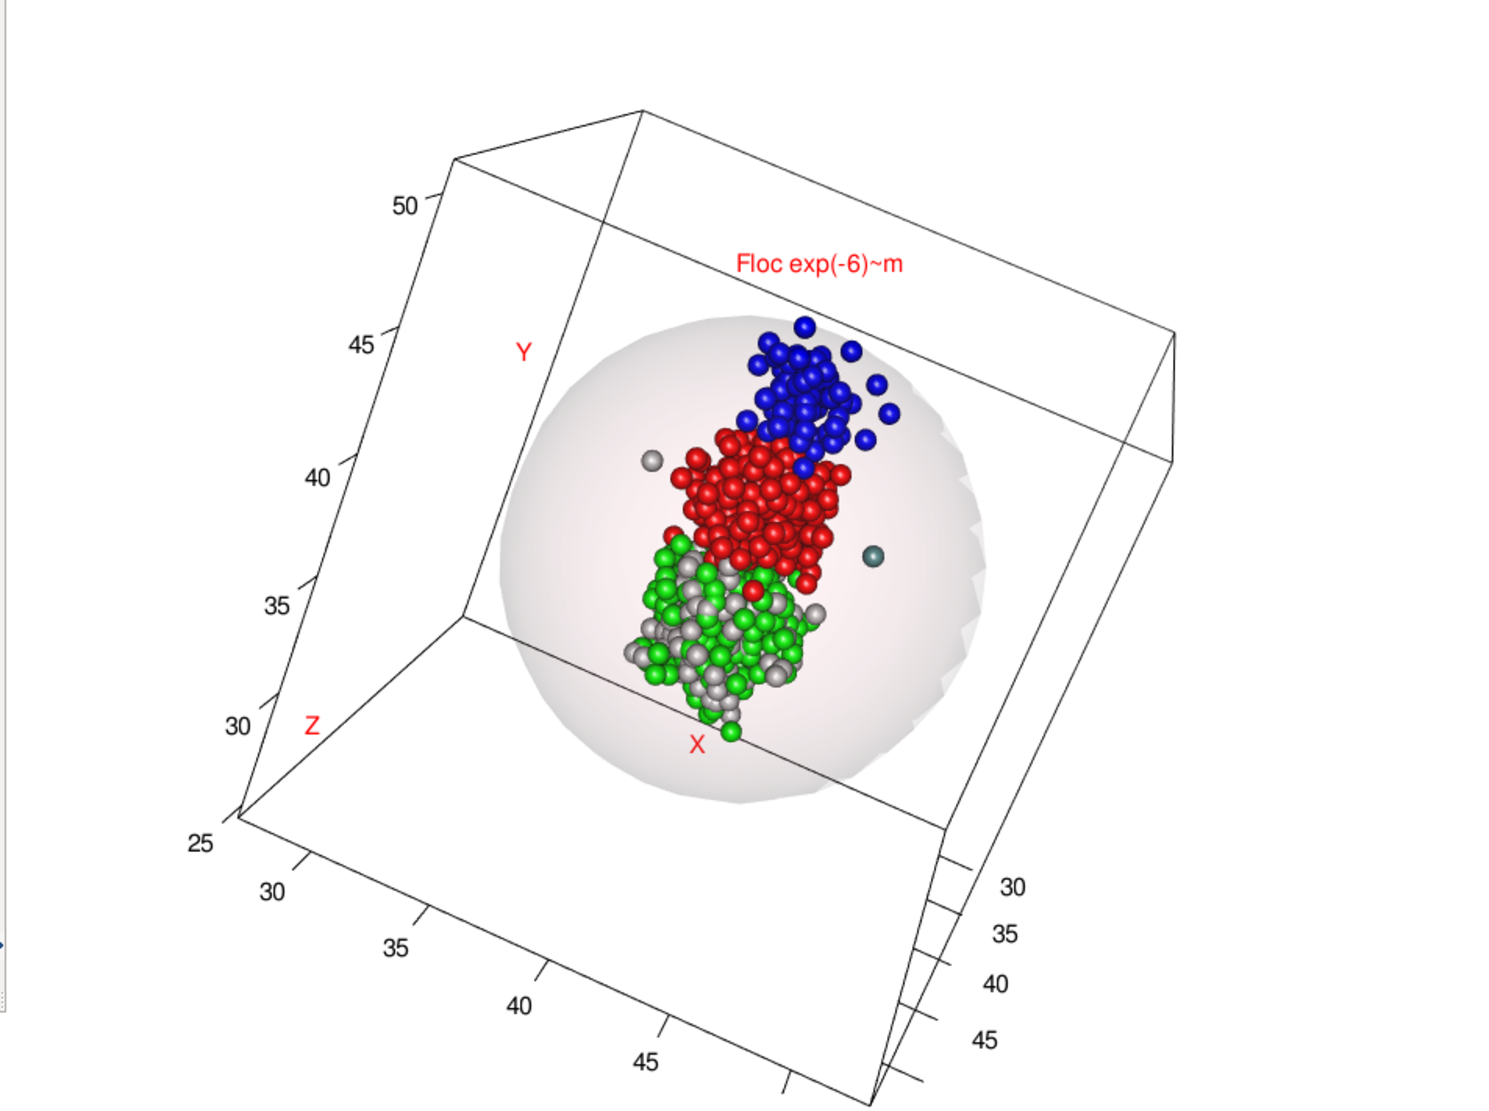
\includegraphics[width=1.1\textwidth]{p2}
\caption[]{LAMMPS floc simulation example.}\label{f1}
\end{figure}

\section{Overview}
Our focus in this section is to highlight what we have done so far, our broad plan and strategy for the upscaling high-level summary from the simulation that will be useful for the project. Since we are developing a statistical algorithm to represent the best relationship between the outputs and inputs (initial conditions) of LAMMPS simulator. It is noted that LAMMPS model is too slow to be run exhaustively at floc level. 
The size and complexity of our problem become increasing because of necessity to make many runs for different input values including repeated runs to incorporate stochasticity and in this case to produce an emulator that predicts reasonable outputs (“perfect” emulator). %This task requires a large number of runs from LAMMPS model.

Our agenda is to apply emulator to adapt and relate LAMMPS model output predictions from an individual particle levels (microscale) to make predictions of an aggregate of particles of varying species called floc/biofilm at mesoscale levels and subsequently, to further transfer the information to macro-level processes of wastewater treatment plants. \citet{l9} earlier reviewed some of the popular techniques for upscaling complex problems while \citet{l4,l8} focused their attention on using an emulator for upscaling hydrological processes and land use management properties.

Firstly, our approach is to condense the long time series outputs of particles of various species from LAMMPS models by spatially aggregating to produce the most relevant outputs in the form of floc aggregates or biofilm. The data compression has the benefit of suppressing or reducing some of the nonlinear response features, simplifying the construction of the emulator. 
Some of highly interested properties at the mesoscale level are the size, shape and structure of biofilm/floc. We shall approximate the floc size using an equivalent diameter and other relevant summaries from the simulation. The floc shall be treated as a ball of a sphere, and we shall estimate the diameter of a sphere that circumscribes its boundary/outline. The center of the sphere will be equivalent to the center of mass of the component particles. See Figure (\ref{diag2}).

Secondly, we shall utilize the Gaussian process emulation in the form of kriging metamodels, combining linear models and Gaussian process emulation of residual data. Our approach here is related to the technique proposed in \citet{l5,l7} and also similar to \citet{l6} who combine GP emulation with a basis representation for calibration of computer models with high dimensional outputs.

\section{Main tasks}
%\subsection{Floc}
The outputs from the LAMMPS will be used to train the proposed emulator. Suppose at time step $t$, the LAMMPS output is written in the form 
\begin{equation}
Y=f(x_t,Y_{t-1})
\end{equation}
Where $Y_{t-1}$ the state vector at the previous time step, $x_t$ are the input at time $t$ which includes the model parameters, forcing and initial conditions.
Consider the current LAMMPS model at particle level as being a model of the floc. We then run the LAMMPS after the model has been recalibrated for floc simulation and simulate the outputs at a microscale. We also summarize the results to a large (mesoscale), e.g., total floc mass 
\begin{equation}
TM_j =\sum^N_i m_{ij},
\end{equation} where $TM$ is the total floc mass at time $j$ for all the species and $m_{ij}$'s are individual particle level mass. 
\begin{itemize}
\item[(1)] The floc aggregates, though irregularly shaped, can approximate as a ball of a sphere made up of particle-level components. The equivalent floc diameter can be estimated by the diameter of the smallest circle that circumscribes the outer edge or sketch of the floc. 
\item[(2)] We shall compute the center of mass $COM$ for the floc aggregate in 3-dimension (and only $Y$ direction for biofilm), for $X$ direction using equation 
\begin{equation}
COM_{x_j}=\frac{\sum^N_i m_{ij} X_{ij}}{TM},
\end{equation}
where $TM$ is as defined above. We will then compute relative distances of each of the particle from the center of mass. The maximum of this distances will form the radius of the outer sphere as shown in Figure (\ref{diag2}).
%\item[(3)] Compute the distance between the $COM$ and each of the particle

\item[(3)] Develop a cheap stochastic emulator of the floc or biofilm using particle scale inputs assuming that the floc is a homogeneous sphere (see \cite{l12} in the NUFEB github repository) for further details.

\item[(4)] Our plan is to focus on the following important properties of floc or biofilm at each time step and develop a time series emulator for the following: 
\begin{itemize}
\item[(i)] Biofilm /floc total mass at each time step
\item[(ii)] Biofilm /floc equivalent diameter at each time step
\item[(iii)] EPS total mass at each time step
\item[(iv)] Total number of particles at each time step
\item[(v)] The mass ratio of individual particle to the total biofilm /floc mass
\item[(vi)] The distribution of floc/ biofilm diameter
\item[(vii*)] The change in the nutrient environment of the floc (defer until the chemistry and hydrodynamics are coupled to the model).
\item[(viii*)] Biofilm surface enlargement (still tricky; need to liase with Prashant/Jaya)
\end{itemize}
\end{itemize}
%Wastewater treatment plant optimization focuses on aggregate outcomes of individual particle-level processes and behavioural rules. 

\begin{figure}[!ht] 
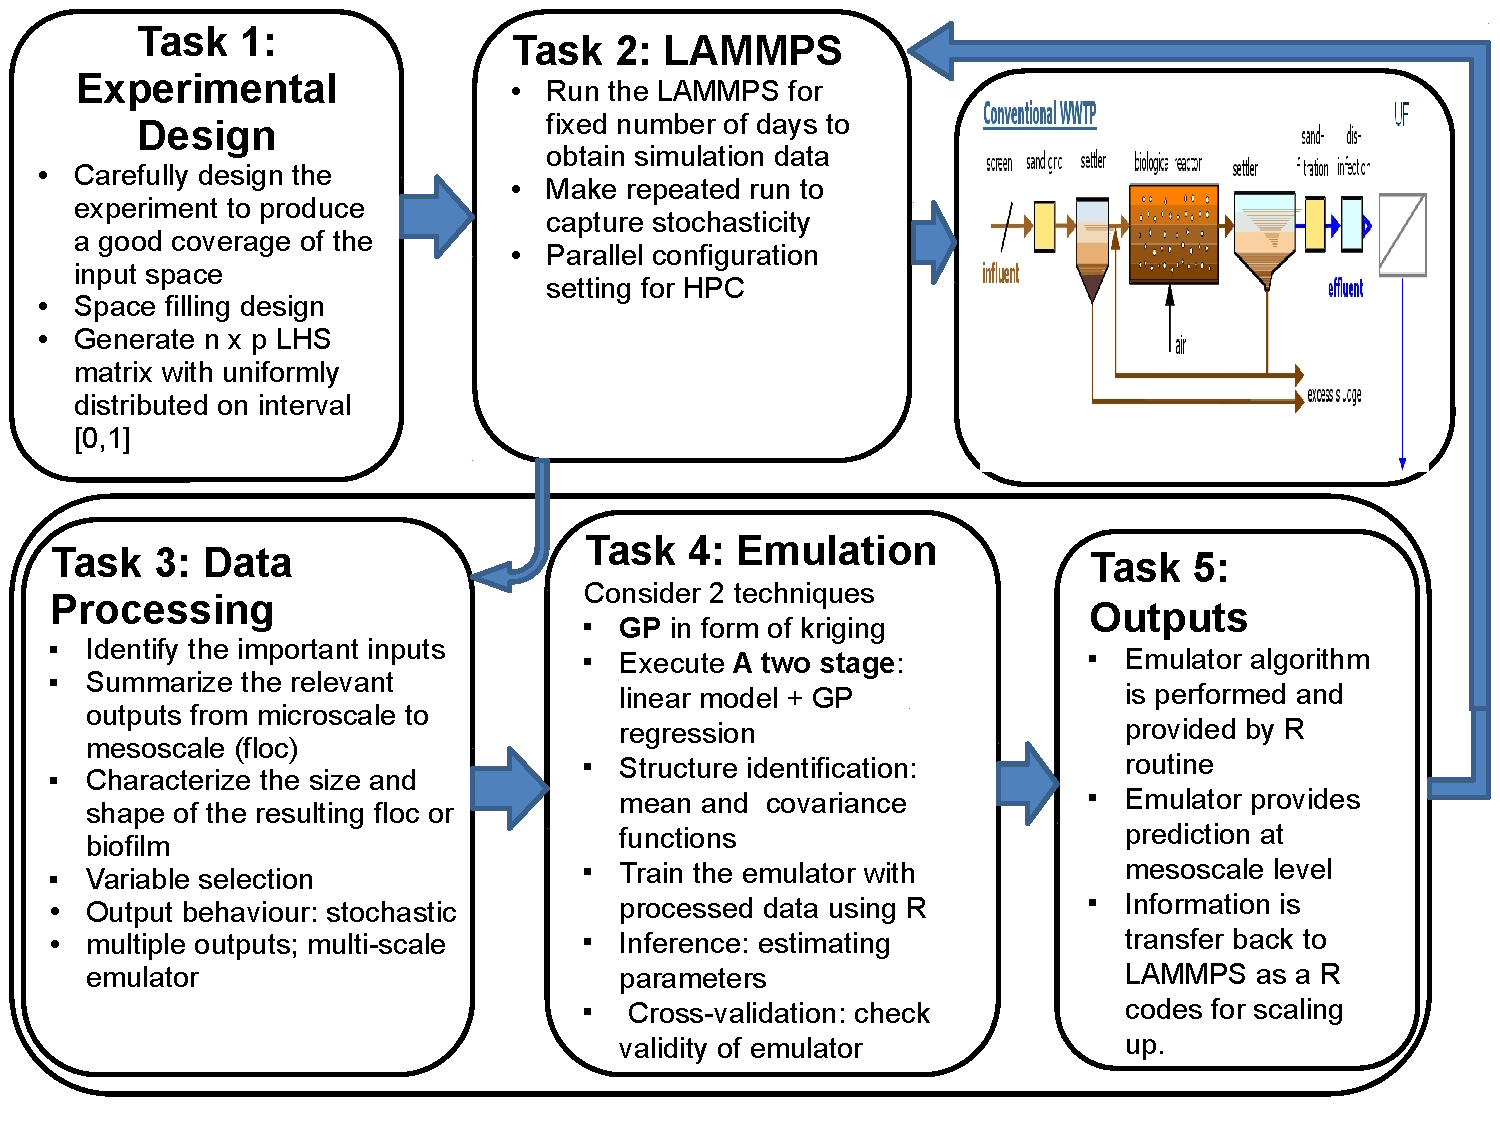
\includegraphics[width=1.1\textwidth]{diagram1}
\caption[]{Schematic diagram showing key stages of LAMMPS emulation.}\label{diag1}
\end{figure}

Presently, some of the listed items above have been implemented for the biofilm, though still open for improvements. A similar idea will be used for modelling floc simulation that we are currently running. Figure (\ref{diag1}) is the schematic for showing key stages in the emulation construction. Task 1 has been completed for both biofilm and floc. We use LHS of 1000 design points for each 25 variables (parameters+ initial conditions) given ($1000 \times 25$), each point is repeated 100 multiple times to incorporate the stochastic variations.
Tasks 2-4 have been completed for the biofilm and Task 2 is being currently implemented for the floc. %The timeline to complete for biofilm was


\section{Emulation procedure}
\begin{itemize}
\item[(1)] Screening: which simulator inputs matter; what are
plausible input range; constraints in the input combinations; 
elicit beliefs about input distributions (we use uniform distributions for all our parameters). 

\item[(2)] Experimental Design: where to run the simulator, we choose points that are reasonably evenly spread throughout the input space to obtain uniform coverage (e.g. LHS). Space-filling design over the entire 25-dimensional input space (from LAMMPS model).  
However, simulation runs are expensive so in our preliminary analysis; we limit the runs to a small number (100 design points and five stochastic repetitions), an array of (100 X 25 X 5) sample points. The LAMMPS model was simulated for ~4 days (345,600 seconds) at a time-step of 2000 seconds, we have~172 runs.

\item[(3)] Data processing: summarize the relevant outputs from microscale to mesoscale (floc), select relevant input variables.

\item[(4)] Emulation: identify the model structure, mean and covariance functions. We build the emulators, estimate parameters and perform cross-validation to check the validity of emulator. 

\item[(5)] Output results: prepare the final emulator code and make some plots.
\end{itemize} 


\begin{thebibliography}{94}
%\cleardoublepage
%\phantomsection
\bibliographystyle{plain}
\bibitem[Marrel et al.(2008)]{l1} Marrel, A., Iooss, B., Van Dorpe, F., \& Volkova, E. (2008). An efficient methodology for modeling complex computer codes with Gaussian processes. {\it Computational Statistics \& Data Analysis}, $52(10), 4731-4744$.

\bibitem[Li et al.(2013)]{l2} Li, Z. L., Zhang, D. J., Lu, P. L., Zeng, S. W., \& Yang, Y.H. (2013). Influencing factors of floc size distribution and fractal dimension of activated sludge. {\it Huan Jing Ke Xue}, $34(10), 3975-3980$.

\bibitem[Jarvis et al.(2005)]{l3} Jarvis, P., Jefferson, B., \& Parsons, S. A. (2005). Measuring floc structural characteristics. {\it Reviews in Environmental Science and Bio/Technology}, $4(1-2), 1-18$.

\bibitem[Frazer et al.(2013)]{l4}  Fraser, C. E., McIntyre, N., Jackson, B. M., \& Wheater, H. S. (2013). Upscaling hydrological processes and land management change impacts using a metamodeling procedure. {\it Water Resources Research}, $49(9), 5817-5833$.

\bibitem[O'Hagan(2006)]{l5} O'Hagan, A. (2006). Bayesian Analysis of Computer Code Outputs: A Tutorial. {\it Reliability Engineering and System Safety}, $91, 1290-1300$.

\bibitem[Higdon et al.(2008)]{l6} Higdon, D., Gattiker, J., Williams, B. \& Rightley, M. (2008). Computer model calibration using high-dimensional output. {\it Journal of the American Statistical Association}, $103, 570-583$.

 \bibitem[Oyebamiji et al.(2015)]{l7} Oyebamiji, O.K., Edwards, N.R., Garthwaite, P.H., Holden, P.B., Schaphoff, S. \& Gerten, D. (2015). Emulating Global Climate Change Impacts on Crop Yields. {\it Statistical Modelling}, 1471082X14568248, first published on January 18, 2015, doi:10.1177/1471082X14568248,\href{http://smj.sagepub.com/content/early/recent}{http://smj.sagepub.com/content/early/recent}
 
 \bibitem[Wheater et al.(2008)]{l8} Wheater, H.S., B. Reynolds, N. McIntyre, M. Marshall, B. Jackson, Z. Frogbrook, I. Solloway, O. J. Francis, and J. Chell (2008). Impacts of upland land management on flood risk: Multi-scale modelling methodology and results from the Pontbren experiment, {\it FRMRC Res. Rep. UR}, 16, 163 pp., Imp. Coll. \& CEH Bangor, London, U.K.
 
 \bibitem[Van et al.(2009)]{l9} Van Oijen, M., Thomson, A., \& Ewert, F. (2009). Spatial upscaling of process-based vegetation models: An overview of common methods and a case-study for the UK. Methods, 1(3).
 
%\bibitem[Jarvis et al.(2005)]{l10} Jarvis, P., Jefferson, B., \& Parsons, S. A. (2005). Measuring floc structural characteristics. Reviews in Environmental Science and Bio/Technology, 4(1-2), 1-18.

\bibitem[Ofiteru et al.(2014)]{l11} Ofiteru, I. D., Bellucci, M., Picioreanu, C., Lavric, V., \& Curtis, T. P. (2014). Multi-scale modelling of bioreactor–separator system for wastewater treatment with two-dimensional activated sludge floc dynamics. {\it Water research}, $50, 382-395$.

\bibitem[LAMMPS Emulation Procedure.pdf (2015)]{l12} Emulation of LAMMPS model outputs (2015). Emulation of LAMMPS model outputs. \href{https://github.com/darrenjw/nufeb/blob/master/LargeScaleModelling/Oluwole/code2/Oluwole3_doc.pdf)}{Oluwole3.pdf}

\end{thebibliography}{}


\end{document}
